\subsection{AI-Assisted Framework Overview}

The development of ecosystem models requires substantial time organizing species into functional groups and determining their interactions. This framework automates these tasks through integration of artificial intelligence with ecological databases. The framework executes four sequential steps: species identification within a region, biological data collection, functional group organization, and interaction determination (Figure~\ref{fig:framework_overview}).

The framework utilizes the Claude-3.5 large language model \citep{Anthropic2024} for data synthesis and ecological analysis. Species identification begins with queries to the Ocean Biodiversity Information System \citep{Grassle1999} and Global Biodiversity Information Facility \citep{GBIF2024}. These queries extract occurrence records, temporal distributions, and abundance data within defined geographical boundaries.

\begin{figure}[htbp]
    \centering
    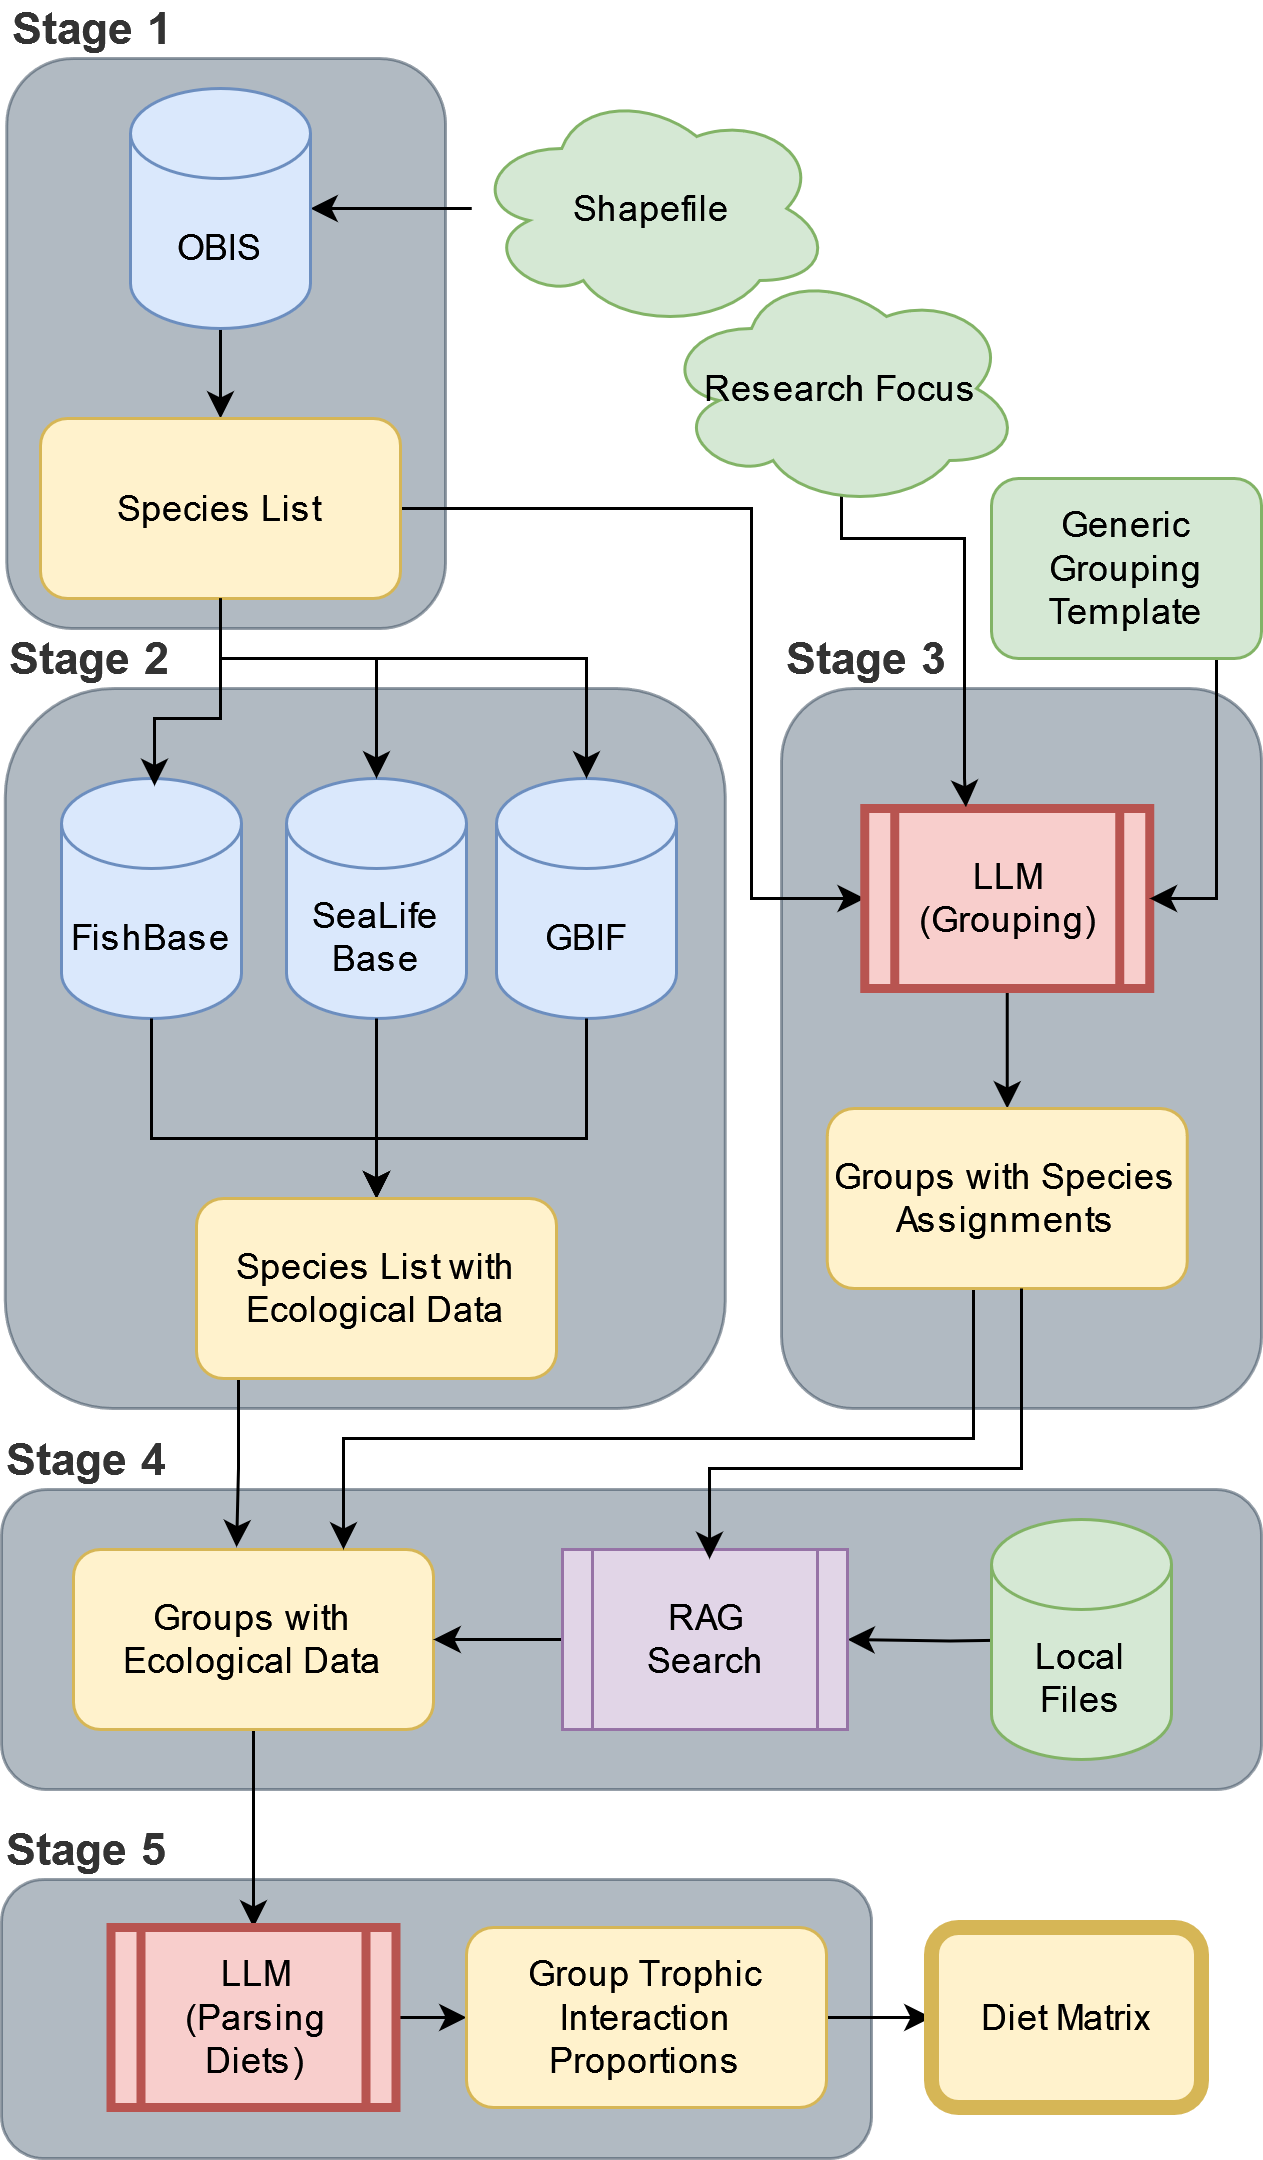
\includegraphics[width=0.5\textwidth]{figures/EwE_AI.drawio.png}
    \caption{Overview of the AI-assisted framework for ecosystem model development. The process consists of four main steps: species identification, biological data collection, functional group organization, and interaction determination. Highlighted stages (functional group organization and interaction determination) undergo systematic validation across multiple iterations. Each step integrates multiple data sources and analytical approaches.}
    \label{fig:framework_overview}
\end{figure}

The biological data collection phase integrates information from multiple sources. FishBase and SeaLifeBase \citep{froese2010fishbase} provide life history traits and ecological parameters. The Ecobase repository \citep{Colleter2015} supplies parameters from existing ecosystem models. Additional data comes from systematic literature searches of regional fisheries reports and peer-reviewed publications, using standardized search terms (e.g., "[species name] AND diet OR feeding OR prey"). Natural language processing extracts relevant ecological information from these documents.

Species grouping employs a vector database (Chroma \citep{Chroma2024}) for characteristic storage and retrieval. The database maintains embedding vectors derived from ecological descriptions, life history traits, and habitat preferences. Analysis of these vectors, combined with ecological rules regarding size classes, feeding guilds, and habitat use, determines functional group assignments. Trophic level estimates from FishBase and SeaLifeBase \citep{froese2010fishbase} validate the ecological coherence of these classifications.

Diet composition analysis merges quantitative records from databases with processed literature data. Food items are extracted from FishBase and SeaLifeBase \citep{froese2010fishbase} databases, supplemented with interaction data from the Global Biotic Interactions (GLOBI) database \citep{Poelen2014}. Each predator-prey interaction includes source documentation and confidence scores based on data quality metrics.

Diet matrix construction implements weighted averaging for prey proportions. Weights derive from data quality metrics including sample size, study recency, and geographical relevance. In cases of sparse direct diet data, the framework estimates trophic interactions based on similar species' preferences and established ecological principles. Each interaction maintains metadata documenting evidence sources and confidence levels.

Parameter estimation prioritizes values from comparable ecosystems and species groups in Ecobase \citep{Colleter2015}. Empirical relationships from literature provide estimates where direct parameters are unavailable. The framework validates all estimates against biological constraints and ecological theory, identifying anomalies for expert review.

Section~\ref{supp:technical_implementation} of the supplementary material contains detailed documentation of all processing steps, including database queries, literature search criteria, and ecological classification rules. The complete codebase and configuration files reside at [GitHub repository URL].
